        
Un \textbf{\og cône de révolution \fg{}} est le solide de l'espace obtenu en faisant tourner un triangle rectangle autour d'un axe, appelé \og axes de révolution \fg{}.Il a:
\begin{itemize}
\item Une base qui est un disque.
\item Une enveloppe latérale qui \og dépliée \fg{}  est un secteur angulaire (voir \og construction du patron d'un cône \fg{}) 
\end{itemize}

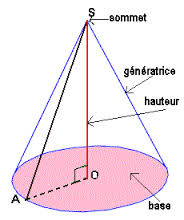
\includegraphics[scale=0.5]{RepS-cone.jpg} 